\begin{abstract}
Despite the recent improvements in admissible heuristic search techniques
in classical planning, it is known that the the exponential growth of
search plateau in A* is unavoidable even under the optimistic assumption.
 % 
We investigate various existing myth on tiebreaking
 strategies and propose simple yet effective methods for improving the
 search performance within plateau.
 % 
 % 
 They do not depend on any particular heuristic, nor
 on multi-heuristic portfolio.
 They work even if the heuristic
 function no longer provides useful information.
 % Moreover, they do not even try to obtain any further information from
 % the domain.
 We empirically evaluate our strategies against state-of-the-art admissible planner.
\end{abstract}

Since the advent of delete-relaxation and abstraction heuristics in
admissible Classical Planning, much of the interest was focused on improving
the accuracy of these heuristic functions to prune more nodes from the
search space.
% 
However, recent work by Helmert and Roger
\shortcite{helmert2008good} claims that, even with an optimistic
assumption of \emph{almost-perfect heuristics}, \astar still has an
exponentially large plateau. They conclude that the further performance
improvement requires the techniques orthogonal to the heuristic
function, such as symmetry breaking, domain reduction, factored planning
etc.

The contribution of this paper is a new class of
tiebreaking strategy for \astar.
It is a heuristic-agnostic improvement and thus 
falls into above category of techniques.
It trivially maintains admissibility because it works only within the
same f-value and does not alter the expansion order wrto f-value.
% such technique.
% tiebreaking strategy for \astar.
% Our tiebreaking strategies fall into this category.

% The attention to the search algorithm itself is relatively small since
% most literature depends on bare \astar.  This was because variations of
% best first search focus on different requirements, such as IDA* on
% linear space, WA*/Lazy-A*/GBFS/EHC on trading speed for optimality, RWA*
% on replanning, etc., and not on improving upon \astar itself.

% maintaining all of its charactristics: memory-greedy yet efficient
% optimal algorithm.

The rest of paper is organized as follows: The next section describes the
preliminary background of \astar.
Next we compares several trivially-simple and well-known tiebreaking
methods on top of Fast Downward to show that even such a small
difference significantly affects the performance on domains with
large plateaus.
Next we propose a novel depth-aware tiebreaking methods and empirically
show that it outperforms previous strategies.
We finally conclude with a discussion on the future work.

\section{Backgrounds and Preliminary}
\label{sec-1}

\subsubparagraph{\astar and perfect heuristics}

\astar is a state of the art algorithm for finding an optimal path in the
search space represented as a graph. 
\astar returns an optimal solution when the heuristic function $h$ is
admissible, i.e., when it never overestimate the true distance to the goal
$h^*$.
% , and the nodes are first ordered according to $f$
% 
Thus, the best possible admissible heuristic function is $h^*$ itself, which is
called \emph{perfect heuristics}. However, computing $h^*$ is PSPACE-Complete,
which is as difficult as solving the problem itself and is not
practical.

%It is known that with a perfect heuristics the planner do not have to
% conduct any search: There are no multiple possibilities that the
% planner should examine on each node.

\emph{Almost perfect} heuristic function $h_c$ is a class of similar
impractical, theoretical functions which is also PSPACE-Complete to
compute \cite{helmert2008good}.  It has a constant error $c$ from the
perfect heuristic $h^*$, i.e., $h_c=h^*-c$.  The important finding by
\citeauthor{helmert2008good} is that even with this intractable and
impractical heuristic function, the number of the nodes in the last
plateau of the search becomes exponentially large as the problem size
increases.  Using this fact, they showed that relying only on the
improvement of the heuristic functions is not fruitful in the near
future, and the researchers should seek the other,
orthorgonal improvement.

These intractable heuristics are of course very hard and expensive to
compute. However, even the practical, tractable heuristic functions
which can be computed in polynomial time, such as \lmcut and IP-based
heuristics, are also very CPU intensive functions that renders the
space-greedy characteristics of \astar negligeble. Also, compared to the
other functions, these functions dominate the search time over the other
factors of planning algorithms, such as node insertion and deletion.

% M\&S ?

\section{Tie Breaking Criteria in \astar}

% Compared to the other algorithms which
% guarantee optimality such as $IDA^*$ \cite{korf1985depth}, \astar requires a large amount of % memory to store the search nodes.

\astar stores the search nodes into two priority queues called an \emph{open list} and a \emph{closed list}, sorted based on $f$ value. While the implementation of the priority queue varies, it has another degree of freedom called tie-breaking, i.e. how to select the next node to open within the same priority.

In the current implementation of the \sota admissible planner Fast Downward (FD) \cite{Helmert2006}, the standard \astar search breaks ties based on $h$, meaning that if two nodes have the same $f$ value, the nodes with smaller $h$ will be selected, favoring the nodes with larger $g$ values (since $f=g+h$). The intension behind this is that the $h$ values are just an \emph{estimate} to the goal, while $g$ values are the \emph{actual} distance from the initial state and more reliable.

Another thing we have to note is that in FD, when even the $h$ values are the same, then the second tiebreaking behavior is basically a FIFO order: The planner selects the nodes that is inserted earlier. 
However, in fact, these tiebreaking methods are not necessary when we are only concerned with  maintaining the optimality. They are just the result of heuristic, ad-hoc selection by humans and have no theoretical background.
% In particular, we first observed that this FIFO order has not legitimate reason to support.

We therefore ran a preliminary experiments on 28 benchmark domains with
1294 problems in total, comparing simple FIFO, LIFO and Random-Order
second-level tiebreaking methods using 30 minutes runtime cutoff with
2GB memory limit.  All experiments below are conducted on Xeon
E5410@2.33GHz CPUs. We observed that even such a slightest difference
can change the performance significantly on some domains, shown in
\reftbl{f-h-coverage}. Due to the space limitation, we show only the
domains where the difference was observed. Full table is available in
the supplemental material.

\refig{f-h-eval} compares the number of
node evaluation (computations of \lmcut) by LIFO, FIFO and Random second
tiebreaking.  According to the figure, LIFO has smaller number of
evaluations than the others in Openstacks, but Random dominates the
others in Cybersec, indicating that there are no dominance relationship
between these three.  \reftbl{f-h-coverage} shows the coverage result
(number of problems solved) by each strategy.

Moreover, we also ran the same experiment but this time without $h$-based
first-level tiebreaking. Results in \reftbl{f-coverage} shows that the
coverage by LIFO-tiebreaking is almost comparable to those with $h$-based
tiebreaking.

% Note that, although LIFO dominated the others, we consider this is just by a coincidence due to our selection of problems, time limit and domains. we \emph{are not trying to claim that any of LIFO or FIFO or Random order dominates the other}. However, there are noticeable performance difference cause by these different tiebreaking strategies.

% \begin{figure}[htbp]
%  \centering
%  \relsize{-2}
%  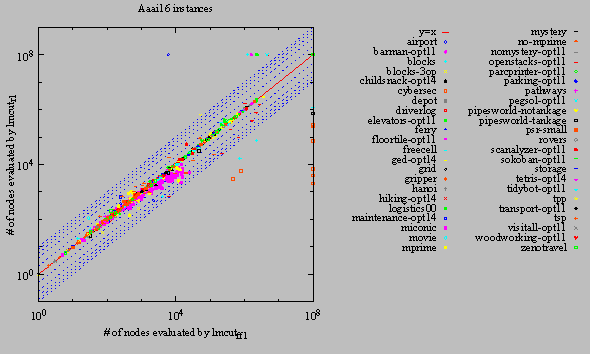
\includegraphics{tables/aaai16-evaluated-lmcut_ff-lmcut_r.pdf}
%  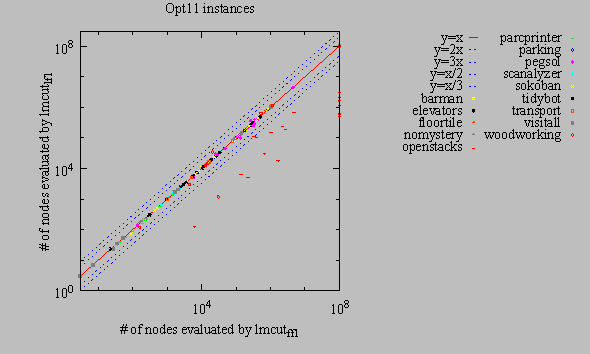
\includegraphics{tables/opt11-evaluated-lmcut_ff-lmcut_lf.pdf}
%  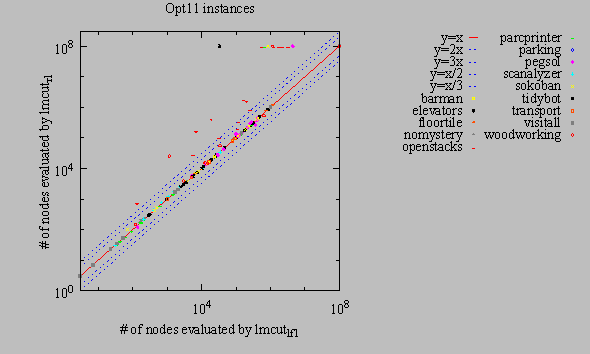
\includegraphics{tables/opt11-evaluated-lmcut_lf-lmcut_r.pdf}
% \caption{Comparison of the number of node evaluations (computations of \lmcut) by FIFO and LIFO tie breaking, on IPC2011 optimal track instance. LIFO order dominates FIFO and Random order especially in openstacks instances, and the gap is more than one the order of 10.}
%  \label{single-eval}
% \end{figure}
% 
% \begin{table}[htbp]
%  \centering
%  \relsize{-2}
%  \begin{tabular}{|c|c|c||c||c||c||c||c||c||c|}
   \hline                        
   &  Domain & \rotatebox[origin=l]{0}{${\mbox{lmcut}}_{\mbox{ffff1}}$}   & \rotatebox[origin=l]{0}{${\mbox{lmcut}}_{\mbox{ff1}}$}   & \rotatebox[origin=l]{0}{${\mbox{lmcut}}_{\mbox{lf1}}$}   & \rotatebox[origin=l]{0}{${\mbox{lmcut}}_{\mbox{r1}}$}   & \rotatebox[origin=l]{0}{${\mbox{lmcut}}_{\mbox{fflf1}}$}   & \rotatebox[origin=l]{0}{${\mbox{lmcut}}_{\mbox{ffr1}}$}   & \rotatebox[origin=l]{0}{${\mbox{lmcut}}_{\mbox{lfr1}}$}   & \rotatebox[origin=l]{0}{${\mbox{lmcut}}_{\mbox{fflfr1}}$}    \\
   \hline                        
\multirow{45}{*}{\rotatebox[origin=c]{90}{}}   &  {\relsize{-1}airport(50)} &  \textbf{28} &  \textbf{28} &  27 &  27 &  \textbf{28} &  \textbf{28} &  27 &  \textbf{28}  \\
   &  {\relsize{-1}barman-opt11-strips(20)} &  \textbf{4} &  \textbf{4} &  \textbf{4} &  3 &  \textbf{4} &  \textbf{4} &  \textbf{4} &  \textbf{4}  \\
   &  {\relsize{-1}blocks(136)} &  24 &  24 &  \textbf{26} &  25 &  \textbf{26} &  \textbf{26} &  \textbf{26} &  \textbf{26}  \\
   &  {\relsize{-1}blocks-3op(30)} &  \textbf{10} &  \textbf{10} &  \textbf{10} &  \textbf{10} &  \textbf{10} &  \textbf{10} &  \textbf{10} &  \textbf{10}  \\
   &  {\relsize{-1}childsnack-opt14-strips(20)} &  \textbf{0} &  \textbf{0} &  \textbf{0} &  \textbf{0} &  \textbf{0} &  \textbf{0} &  \textbf{0} &  \textbf{0}  \\
   &  {\relsize{-1}cybersec(19)} &  2 &  2 &  3 &  \textbf{9} &  3 &  \textbf{9} &  8 &  8  \\
   &  {\relsize{-1}depot(22)} &  \textbf{7} &  \textbf{7} &  \textbf{7} &  \textbf{7} &  6 &  6 &  \textbf{7} &  \textbf{7}  \\
   &  {\relsize{-1}driverlog(20)} &  \textbf{13} &  \textbf{13} &  \textbf{13} &  \textbf{13} &  \textbf{13} &  \textbf{13} &  \textbf{13} &  \textbf{13}  \\
   &  {\relsize{-1}elevators-opt11-strips(20)} &  \textbf{17} &  \textbf{17} &  16 &  16 &  15 &  14 &  14 &  14  \\
   &  {\relsize{-1}ferry(30)} &  \textbf{30} &  \textbf{30} &  \textbf{30} &  \textbf{30} &  \textbf{30} &  \textbf{30} &  \textbf{30} &  \textbf{30}  \\
   &  {\relsize{-1}floortile-opt11-strips(20)} &  \textbf{6} &  \textbf{6} &  \textbf{6} &  \textbf{6} &  \textbf{6} &  \textbf{6} &  \textbf{6} &  \textbf{6}  \\
   &  {\relsize{-1}freecell(80)} &  \textbf{13} &  \textbf{13} &  12 &  \textbf{13} &  \textbf{13} &  \textbf{13} &  \textbf{13} &  \textbf{13}  \\
   &  {\relsize{-1}ged-opt14-strips(20)} &  \textbf{15} &  \textbf{15} &  \textbf{15} &  \textbf{15} &  \textbf{15} &  \textbf{15} &  \textbf{15} &  13  \\
   &  {\relsize{-1}grid(5)} &  \textbf{2} &  \textbf{2} &  \textbf{2} &  \textbf{2} &  \textbf{2} &  \textbf{2} &  \textbf{2} &  \textbf{2}  \\
   &  {\relsize{-1}gripper(20)} &  \textbf{6} &  \textbf{6} &  \textbf{6} &  \textbf{6} &  \textbf{6} &  \textbf{6} &  \textbf{6} &  \textbf{6}  \\
   &  {\relsize{-1}hanoi(30)} &  \textbf{12} &  \textbf{12} &  \textbf{12} &  \textbf{12} &  \textbf{12} &  11 &  \textbf{12} &  \textbf{12}  \\
   &  {\relsize{-1}hiking-opt14-strips(20)} &  \textbf{8} &  \textbf{8} &  \textbf{8} &  \textbf{8} &  \textbf{8} &  \textbf{8} &  \textbf{8} &  \textbf{8}  \\
   &  {\relsize{-1}logistics00(199)} &  \textbf{21} &  \textbf{21} &  20 &  \textbf{21} &  \textbf{21} &  \textbf{21} &  20 &  \textbf{21}  \\
   &  {\relsize{-1}maintenance-opt14-adl(5)} &  \textbf{5} &  \textbf{5} &  \textbf{5} &  \textbf{5} &  \textbf{5} &  \textbf{5} &  \textbf{5} &  \textbf{5}  \\
   &  {\relsize{-1}miconic(150)} &  \textbf{140} &  \textbf{140} &  \textbf{140} &  \textbf{140} &  \textbf{140} &  \textbf{140} &  \textbf{140} &  \textbf{140}  \\
   &  {\relsize{-1}movie(30)} &  \textbf{30} &  \textbf{30} &  \textbf{30} &  \textbf{30} &  \textbf{30} &  \textbf{30} &  \textbf{30} &  \textbf{30}  \\
   &  {\relsize{-1}mprime(35)} &  \textbf{22} &  \textbf{22} &  \textbf{22} &  \textbf{22} &  \textbf{22} &  21 &  \textbf{22} &  \textbf{22}  \\
   &  {\relsize{-1}mystery(30)} &  16 &  16 &  \textbf{17} &  16 &  \textbf{17} &  16 &  16 &  \textbf{17}  \\
   &  {\relsize{-1}no-mprime(35)} &  \textbf{22} &  \textbf{22} &  \textbf{22} &  \textbf{22} &  \textbf{22} &  \textbf{22} &  \textbf{22} &  \textbf{22}  \\
   &  {\relsize{-1}nomystery-opt11-strips(20)} &  \textbf{14} &  \textbf{14} &  \textbf{14} &  \textbf{14} &  \textbf{14} &  \textbf{14} &  \textbf{14} &  \textbf{14}  \\
   &  {\relsize{-1}openstacks-opt11-strips(20)} &  11 &  11 &  \textbf{19} &  10 &  18 &  10 &  16 &  16  \\
   &  {\relsize{-1}parcprinter-opt11-strips(20)} &  \textbf{13} &  \textbf{13} &  \textbf{13} &  \textbf{13} &  \textbf{13} &  \textbf{13} &  \textbf{13} &  \textbf{13}  \\
   &  {\relsize{-1}parking-opt11-strips(20)} &  \textbf{1} &  \textbf{1} &  \textbf{1} &  \textbf{1} &  \textbf{1} &  \textbf{1} &  \textbf{1} &  \textbf{1}  \\
   &  {\relsize{-1}pathways(30)} &  \textbf{5} &  \textbf{5} &  \textbf{5} &  \textbf{5} &  \textbf{5} &  \textbf{5} &  \textbf{5} &  \textbf{5}  \\
   &  {\relsize{-1}pegsol-opt11-strips(20)} &  \textbf{17} &  \textbf{17} &  \textbf{17} &  16 &  \textbf{17} &  16 &  16 &  16  \\
   &  {\relsize{-1}pipesworld-notankage(50)} &  \textbf{16} &  \textbf{16} &  \textbf{16} &  \textbf{16} &  \textbf{16} &  \textbf{16} &  \textbf{16} &  \textbf{16}  \\
   &  {\relsize{-1}pipesworld-tankage(50)} &  \textbf{9} &  8 &  \textbf{9} &  \textbf{9} &  \textbf{9} &  8 &  8 &  8  \\
   &  {\relsize{-1}psr-small(50)} &  \textbf{48} &  \textbf{48} &  \textbf{48} &  \textbf{48} &  \textbf{48} &  \textbf{48} &  \textbf{48} &  \textbf{48}  \\
   &  {\relsize{-1}rovers-large(40)} &  \textbf{7} &  \textbf{7} &  \textbf{7} &  \textbf{7} &  \textbf{7} &  \textbf{7} &  \textbf{7} &  \textbf{7}  \\
   &  {\relsize{-1}scanalyzer-opt11-strips(20)} &  \textbf{9} &  \textbf{9} &  \textbf{9} &  \textbf{9} &  \textbf{9} &  \textbf{9} &  8 &  \textbf{9}  \\
   &  {\relsize{-1}sokoban-opt11-strips(20)} &  19 &  \textbf{20} &  \textbf{20} &  \textbf{20} &  \textbf{20} &  \textbf{20} &  \textbf{20} &  19  \\
   &  {\relsize{-1}storage(30)} &  \textbf{15} &  \textbf{15} &  \textbf{15} &  \textbf{15} &  \textbf{15} &  \textbf{15} &  \textbf{15} &  \textbf{15}  \\
   &  {\relsize{-1}tetris-opt14-strips(17)} &  \textbf{3} &  \textbf{3} &  \textbf{3} &  \textbf{3} &  \textbf{3} &  \textbf{3} &  \textbf{3} &  \textbf{3}  \\
   &  {\relsize{-1}tidybot-opt11-strips(20)} &  \textbf{13} &  \textbf{13} &  \textbf{13} &  \textbf{13} &  \textbf{13} &  \textbf{13} &  \textbf{13} &  \textbf{13}  \\
   &  {\relsize{-1}tpp(30)} &  \textbf{6} &  \textbf{6} &  \textbf{6} &  \textbf{6} &  \textbf{6} &  \textbf{6} &  \textbf{6} &  \textbf{6}  \\
   &  {\relsize{-1}transport-opt11-strips(20)} &  \textbf{6} &  \textbf{6} &  \textbf{6} &  \textbf{6} &  \textbf{6} &  \textbf{6} &  \textbf{6} &  \textbf{6}  \\
   &  {\relsize{-1}tsp(30)} &  \textbf{30} &  \textbf{30} &  \textbf{30} &  \textbf{30} &  \textbf{30} &  \textbf{30} &  \textbf{30} &  \textbf{30}  \\
   &  {\relsize{-1}visitall-opt11-strips(20)} &  \textbf{10} &  \textbf{10} &  \textbf{10} &  \textbf{10} &  \textbf{10} &  \textbf{10} &  \textbf{10} &  \textbf{10}  \\
   &  {\relsize{-1}woodworking-opt11-strips(20)} &  8 &  8 &  \textbf{9} &  8 &  8 &  8 &  8 &  8  \\
   &  {\relsize{-1}zenotravel(20)} &  \textbf{12} &  \textbf{12} &  \textbf{12} &  \textbf{12} &  \textbf{12} &  \textbf{12} &  \textbf{12} &  \textbf{12}  \\
   \hline                        
   &  Sum &  725 &  725 &  \textbf{735} &  729 &  734 &  726 &  731 &  732 \\
\hline
\end{tabular}

%  \caption{Preliminary experiments comparing the performance of FIFO, LIFO and Random second-level tiebreaking using Fast Downward. Each cell denotes the problem solved with 5 minutes runtime, 2GB memory limitation. \textbf{Boldface} denotes the case where it achieved the best result among configurations. LIFO tiebreaking was obtained by modifying the TieBreakingOpenList in FD. Both FIFO and LIFO use $[g+h,h]$ as a sorting criteria, where $h=$\lmcut. For Random tiebreaking, we implemented a so-called ``random heuristics'' $r$, which always returns a random value, then used it as the second tiebreaking, i.e., $[g+h,h,r]$. The seed is initialized to 1.}
%  \label{single-coverage}
% \end{table}

We also observed such differences occur especially in the problems which
have the huge search plateau, i.e., the problems where the heuristic
function is not informative and the planner relies heavily on the
tiebreaking criteria.  \refig{plateau-f-h} shows the initial size of the
tiebreaking bucket in which the goal node was found, compared to the
total amount of search effort measured by node evaluation. It uses FIFO
as the second tiebreaking criteria.  The nodes in a same bucket shares
the same $[f,h]$ value, therefore the planner cannot be guided by the
heuristic functions within this bucket. In Openstacks and Cyberspecs, the planner
appears to spend almost half the time on searching through the last
plateau, and those domains are greatly affected by the difference in the
second tiebreaking such as LIFO, FIFO or Random, according to the
previous figures.
In \refig{plateau-h}, we also compared the similar statistics where the $h$-based tiebreaking is disabled. We observed that much higher amount of effort is spent on the plateau based on single-element tiebreaking vector $[f]$.

% \begin{figure}[htbp]
%  \centering
%  \relsize{-2}
%  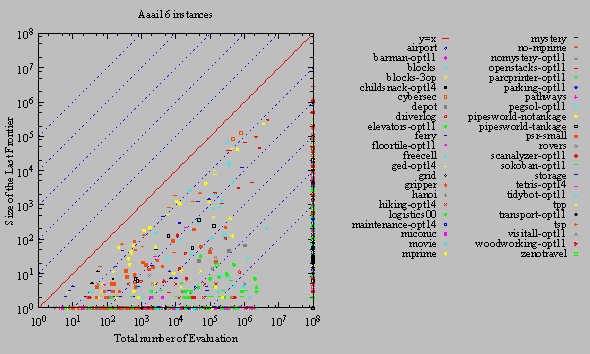
\includegraphics{tables/aaai16-front-vs-evaluated.pdf}
%  \caption{Comparison of the size of the search plateau compared to the total evaluation. Data were obtained by the result of standard FIFO tiebreaking on the standard benchmark instances. Both axes are logarithmic. Each dotted line represents 10x, 100x ... lines.  Openstacks,  clearly has the large plateaus.}
%  \label{plateau-h}
% \end{figure}
% 
% \begin{figure}[htbp]
%  \centering
%  \relsize{-2}
%  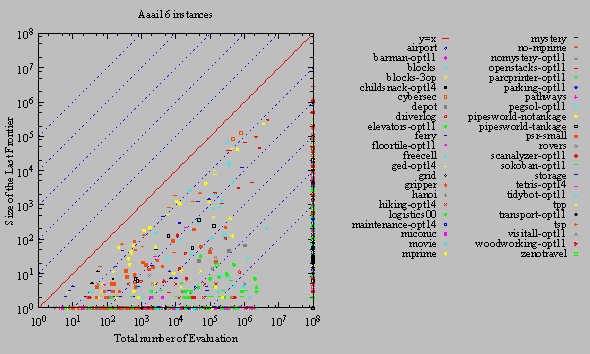
\includegraphics{tables/aaai16-front-vs-evaluated.pdf}
%  \caption{Comparison of the size of the search plateau compared to the total evaluation. Data were obtained by the result of running \astar on the standard benchmark instances, with FIFO but without the tiebreaking by $h$. Both axes are logarithmic. Each dotted line represents 10x, 100x ... lines.}
%  \label{plateau-f}
% \end{figure}


We can have several important observations from these results.  Firstly, in a plateau, \textbf{the heuristic functions are not used at all, nor the search is guided at all}. This observation holds even if we combine several nondominating heuristics for tie breaking e.g. \lmcut and M\&S.  It is still possible that a plateau is encountered, since their combination is not a perfect heuristics yet!

Secondly, such a plateau is known to be inevitable even if we have an almost perfect heuristics $h_c$, and it is impossible to improve upon $h_c$ --- if it could, the result would be a perfect heuristics or an inadmissible heuristics. Therefore, this problem \textbf{cannot be solved by improving the heuristic accuracy, which is the currently dominating meta-strategy to improve the planner performance.}  Note that combining multiple heuristic functions by taking their maximum is still an attempt to improve the accuracy, therefore it does not solve this problem.

Thirdly, there is no legitimate reason which supports each tiebreaking strategy. \textbf{$h$ and FIFO are just heuristically chosen by the implementer of the planner.} Nor are there any reason to choose LIFO, or Random tie breaking. Notably, it iscan be easily inferred that the different seed value of a Random tiebreaking yield the different search behavior and different result. (In all of our experiment we fixed the seed to 1.)

% Based on these observation, the next step we have taken is to develop a new
% portfolio-based multi-tiebreaking strategy \textbf{which is orthogonal to
% the approach of improving the heuristic accuracy.}

\section{Domains with Large Plateau}

Limiting our observation only to 2 domains is not a promising
result. Therefore, we created several domains where the \sota heuristic
functions fail to provide a menaingful guidance.

One important characteristics shared by Openstacks and Cybersec is that they both
have large number of zero-cost actions. In such situations, both LMcut
and M\&S fail to find a meaningful heuristic estimate because LMcut fails to
find a good cost partitioning with non-zero values, and most edges in the abstraction space of
M\&S have zero costs.

We therefore modified various domains to have zero-cost actions.
For example, miconic-up is a domain which minimizes the energy
consumption caused by ``up'' action, which moves the elevator up, and
ignores other factors.  Another example is driverlog-fuel, where only
the ``drive'' action has cost 1 and all other actions are zero-cost.
This in fact reflects the practical application compared to the original
unit-cost domains where driving and manual labor is equally accounted.
Oddly, although some planners have options which treats actions as if
they are unit-costs, and describe such options as ``inadmissible'',
solving domains which are unit-cost by origin is not called
``inadmissible''. Above domain modification addresses this problem.



\section{Related Work}
\label{sec-4}

\emph{Symmetry Breaking} \cite{Fox1998,pochter2011exploiting,domshlak2013symmetry} is the search technique that tries to prune the states with symmetric paths. \emph{Partial Order Reduction}, \emph{Strong Stubbern Sets} and \emph{Expansion Core} are also the techniques which prune the intermediate states that reach to the same goal using the different orders of same actions. \emph{Dominance Pruning} \cite{erol1994} is a technique which exploits additional information from the problem after the heuristics are computed. Instead of computing the absolute distance, it  proves if a state is strictly relatively better than the other nodes. Since path similarity is weaker than symmetry or other criteria, our approach does not prune states, and instead just delay the expansion within the same f-value.

LA*

\section{Conclusion}

In this paper, we proposed two novel diversity-aware tie-braking methods for the admissible search using \astar. We empirically showed that they improve the performance on various domains, and they are heuristic-agnostic improvements. We showed that they have a significant impact on the final step of the search in large plateau.
 % when the distribution of optimal solutions is not uniform within the open list.
% We also showed that this nonuniform distribution still appears when we have almost-perfect % heuristics.

Our method differs from the other pruning techniques such as symmetry breaking, dominance pruning or partial-order-pruning because we actually do not prune any states, nor from the other general improvements in the heuristic accuracy because we just change the expansion order within the same $f$.
